%!TEX TX-program = xelatex
\documentclass[8pt]{article}

\usepackage{ctex}
\usepackage{graphicx}
\usepackage{enumitem}
\usepackage{geometry}
\usepackage{amsmath}
\usepackage{amssymb}
\usepackage{amsfonts}
\usepackage{tikz}
\usetikzlibrary{positioning}
\usetikzlibrary{svg.path}
\usepackage{xcolor}

\graphicspath{ {./images/} }

\title{2 等式与不等式}
\author{高一(6)班\ 邵亦成\ 26号}
\date{2021年10月21日}

\geometry{a4paper, scale=0.8}

\setcounter{section}{1}

\begin{document}

	\maketitle

	\section{等式与不等式}
		\subsection{等式与不等式的性质}
			\textbf{等式}:用符号$=$连接起来的两个式子.

			\textbf{等式的性质}:传递性,加法性质,乘法性质.

			\textbf{等式的加法性质}:$a=b\Leftrightarrow a+c=b+c$.

			\textbf{等式的乘法性质}:$a=b\Rightarrow ac=bc$,$ac=bc \textbf{ and } c\neq 0 \Rightarrow a=b$.

			\textbf{方程}:含有未知数的等式.

			\textbf{方程的解}:使等式成立的未知数的值.

			\textbf{根}:一元方程的解.

			\textbf{重根}:一元整式方程的相等的根.

			\textbf{方程的解集}:以方程的所有解为元素组成的集合. 重根在解集中只出现一次.

			\textbf{不等式}:用不等号连接的式子.

			\textbf{不等号}:$<, >, \leq, \geq$.

			\textbf{不等式的基本性质}:$b>a \Leftrightarrow b-a>0$,$b<a \Leftrightarrow b-a<0$,$b=a \Leftrightarrow b-a=0$.

			\textbf{不等式的方向改变}:$a>b \Leftrightarrow b<a$.

			\textbf{不等式的性质}:传递性,加法性质,乘法性质.

			\textbf{不等式的加法性质}:$a>b \Leftrightarrow a+c>b+c.$

			\textbf{不等式的乘法性质}:$c>0, a>b\Leftrightarrow ac>bc$;$c<0, a>b\Leftrightarrow ac<bc$.

			\textbf{不等式的常用性质}:

			\begin{enumerate}[label=(\arabic*)]
				\item $a>b \text{ and } c>d \Rightarrow a+c>b+d.$
				\item $a>b>0 \Leftrightarrow \frac{1}{b}>\frac{1}{a}>0.$
				\item $a<b<0 \Leftrightarrow \frac{1}{b}<\frac{1}{a}<0.$
				\item $a>b>0, c>d>0 \Rightarrow ac>bd>0.$
				\item $n\in\mathbf{N}^{*}, a>b>0 \Rightarrow a^n>b^n>0.$
				\item $n\in\mathbf{N}^{*}, a>0, b>0, a^n>b^n>0 \Rightarrow a>b>0.$
			\end{enumerate}

			\textbf{不等式的解}:使不等式成立的未知数的值.

			\textbf{不等式的解集}:以不等式的所有解为元素组成的集合.

			~\\

			\textbf{例一}:若$30<x<42, 16<y<24$,求$x+y, x-2y, \frac{x}{y}$的范围.
				~\\

				$30+16<x+y<42+24 \Rightarrow 46<x+y<66.$

				$-48<-2y<-32 \Rightarrow -18<x-2y<10.$

				$\displaystyle \frac{1}{24}<\frac{1}{y}<\frac{1}{16} \Rightarrow \frac{5}{4}<\frac{x}{y}<\frac{21}{8}.$

				\textcolor{red}{\textbf{总结:不等式具有简单加、减、乘、除的规律,但应注意运算数的符号.}}

			~\\

			\textbf{例二}:$2<x+y<4, 1<x-y<2$. 求$x, y, 4x-2y$的范围.
				~\\

				$\displaystyle 3<2x<6 \Rightarrow \frac{3}{2}<x<3.$

				$\displaystyle 0<2y<3 \Rightarrow 0<y<\frac{3}{2}.$

				\textcolor{red}{$6<4x<12, -3<-2y<0 \Rightarrow 3<4x-2y<12.$ \textbf{错误!}}

				$4x-2y=1\times(x+y)+3\times(x-y) \Rightarrow 5<4x-2y<10.$

				\textcolor{red}{\textbf{总结:不能使用中间结论推出,因为$x$与$y$取到极值的条件不同. 应直接使用原条件(两个不相干的,能同时取到极值的代数式)进行计算.}}

		\newpage
		\subsection{不等式的求解}
			\subsubsection{一元一次不等式的求解}
				\textbf{例一}:解关于$x$的不等式$m(x+2)>x+m$.
					~\\

					$(m-1)x>-m$,分三类讨论.

					\begin{enumerate}[label=$\arabic*^{\circ}$]
						\item $\displaystyle m-1=0\Rightarrow m=1 \Rightarrow x\in\mathbf{R}$.
						\item $\displaystyle m-1>0\Rightarrow m>1 \Rightarrow x\in\left(\frac{m}{1-m}, +\infty\right)$
						\item $\displaystyle m-1<0\Rightarrow m<1 \Rightarrow x\in\left(-\infty, \frac{m}{1-m}\right)$
					\end{enumerate}

					综上,当$m\in(-\infty, 1)$时,解集为$\displaystyle\left(-\infty, \frac{m}{1-m}\right)$;当$m=1$时,解集为$\mathbf{R}$;当$m\in(1, +\infty)$时,解集为$\displaystyle\left(\frac{m}{1-m}, +\infty\right).$

					\textcolor{red}{\textbf{总结:解含参不等式应对参数进行正、负的讨论(不等式的乘法性质).}}

			\subsubsection{一元二次不等式的求解}
				\textbf{一元二次不等式}:设$a, b, c\in \mathbf{R}, a\neq 0$. 形如$ax^2+bx+c>0 (<0, \geq 0, \leq 0)$的不等式.

				\textbf{一元二次不等式的求解}:(1) 化为二次项系数$>0$的一元二次不等式 (2) 解对应一元二次方程 (3) 根据图像写解集:大于取两边,小于取中间.

				\textbf{一元二次不等式的解集}:假设$a>0, \Delta=b^2-4ac$,则有:

				$$
				\begin{array}{cccc}
					&\Delta>0&\Delta=0&\Delta<0\\
			    	ax^2+bx+c=0&\{x_1, x_2\} (x_1 < x_2)&\{x_1\}&\emptyset\\
			    	ax^2+bx+c>0&(-\infty, x_1)\cup(x_2, +\infty)&(-\infty, x_1)\cup(x_1, +\infty)&\mathbf{R}\\
			    	ax^2+bx+c\geq0&(-\infty, x_1]\cup[x_2, +\infty)&\mathbf{R}&\mathbf{R}\\
			    	ax^2+bx+c<0&(x_1, x_2)&\emptyset&\emptyset\\
			    	ax^2+bx+c\leq0&[x_1, x_2]&\{x_1\}&\emptyset\\
			    	y=ax^2+bx+c&
			    	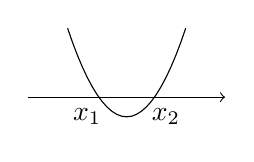
\begin{tikzpicture}[scale=0.25]
			    		\draw[black, ->] (-5, 0)--(5, 0);
			    		\draw[black, domain=-3:3] plot(\x,0.5*\x*\x-1) node at (-2, -1){$x_1$} node at (2, -1){$x_2$};
			    	\end{tikzpicture}&
			    	\begin{tikzpicture}[scale=0.25]
			    		\draw[black, ->] (-5, 0)--(5, 0);
			    		\draw[black, domain=-3:3] plot(\x,0.5*\x*\x) node at (0, -1){$x_1$};
			    	\end{tikzpicture}&
			    	\begin{tikzpicture}[scale=0.25]
			    		\draw[black, ->] (-5, 0)--(5, 0);
			    		\draw[black, domain=-3:3] plot(\x,0.5*\x*\x+1);
			    	\end{tikzpicture}\\
				\end{array}
				$$

				~\\

				\textbf{例一}:设$k\in\mathbf{R}$,解关于$x$的不等式$kx^2-(1-k^2)x+k>0$.

					\begin{enumerate}[label=$\arabic*^{\circ}$]
						\item $k=0 \Rightarrow x\in(-\infty, 0).$
						\item $k\neq 0$, $(kx-1)(x-k)>0$, 对应二次方程两根为$\displaystyle \frac{1}{k}, k.$ $\displaystyle \frac{1}{k}-k=\frac{1-k^2}{k}.$
							\begin{enumerate}[label=$2.\arabic*^{\circ}$]
								\item $k>0$
									\begin{enumerate}[label=$2.1.\arabic*^{\circ}$]
										\item $k>1$, $\displaystyle \frac{1}{k}<k, x\in\left(-\infty, \frac{1}{k}\right)\cup\left(k, +\infty\right).$
										\item $k=1$, $\displaystyle \frac{1}{k}=k, x\in\left(-\infty, 1\right)\cup\left(1, +\infty\right).$
										\item $0<k<1$, $\displaystyle \frac{1}{k}=k, x\in\left(-\infty, k\right)\cup\left(\frac{1}{k}, +\infty\right).$
									\end{enumerate}
								\item $k<0$
									\begin{enumerate}[label=$2.2.\arabic*^{\circ}$]
										\item $-1<k<0$, $\displaystyle \frac{1}{k}<k, x\in\left(\frac{1}{k},k\right).$
										\item $k=-1$, $\displaystyle \frac{1}{k}=k, x\in\emptyset.$
										\item $k<-1$, $\displaystyle \frac{1}{k}=k, x\in\left(k, \frac{1}{k}\right).$
									\end{enumerate}
							\end{enumerate}
					\end{enumerate}

					综上,当$k\in(-\infty, -1)$时,解集为$\displaystyle\left(k, \frac{1}{k}\right)$;当$k=-1$时,解集为$\displaystyle\emptyset$;当$k\in(-1, 0)$时,解集为$\displaystyle\left(\frac{1}{k}, k\right)$;当$k=0$时,解集为$\displaystyle\left(-\infty, 0\right)$;当$k\in(0, 1)$时,解集为$\displaystyle \left(-\infty, k\right)\cup\left(\frac{1}{k}, +\infty\right)$;当$k=1$时,解集为$\left(-\infty, 1\right)\cup\left(1, +\infty\right)$;当$k\in(1, +\infty)$时,解集为$\displaystyle \left(-\infty, \frac{1}{k}\right)\cup\left(k, +\infty\right)$.

					\textcolor{red}{\textbf{总结:(1) 解含参一元二次不等式首先对二次项的-, 0, +进行讨论 (2) 0化为含参一次不等式,-化为+ (3) 分类讨论两根大小,分段写解集.}}

				~\\

				\textbf{例二}:一元二次不等式组$\displaystyle\left\{\begin{array}{rclc}2x^2-x-1&>&0&\textcircled{1}\\2x^2+(2a+5)x+5a&<&0&\textcircled{2}\end{array}\right.$整数解的集合为$\{-2, -1\}$. 求$a$的范围.
					~\\

					由\textcircled{1}: $(2x+1)(x-1)>0 \Rightarrow x\in\left(-\infty, -\frac{1}{2}\right)\cup(1, +\infty).$

					由\textcircled{2}: $(2x+5)(x+a)<0,$

					当$a<\frac{5}{2}$, $x\in\left(-\frac{5}{2}, -a\right)$;当$a=\frac{5}{2}$, $x\in\emptyset$;当$a>\frac{5}{2}$, $x\in\left(-a, -\frac{5}{2}\right)$.

					$\because$整数解的集合为$\{-2, -1\}$

					$\therefore a<\frac{5}{2}$

					$\therefore -a>-1 \textbf{ and } -a \leq 2$

					$\therefore a\in [-2, 1).$

					\textcolor{red}{\textbf{总结:整数解的集合即为解集交整数集,端点情况单独考虑,绘制数轴求解.}}

				~\\

				\textbf{例三}:已知$\forall x \in \mathbf{R}: \displaystyle \frac{ax^2+2ax+2}{x^2+2x+3}<2$恒成立,求$a$的范围.
					~\\

					$\because x^2+2x+3=(x+1)^2+1\geq 1>0$

					$\therefore ax^2+2ax+2<2(x^2+2x+3)$

					$\therefore (a-2)x^2+(2a-4)x-4<0$对$x\in \mathbf{R}$恒成立.

					\begin{enumerate}[label=$\arabic*^{\circ}$]
						\item $a-2=0, a=2, -4<0$符合题意.
						\item $a-2\neq 0, a\neq 2, $有:
							$\displaystyle\left\{\begin{array}{rcl}a-2&<&0\\\Delta&<&0\end{array}\right.\Rightarrow a\in(-2, 2).$
					\end{enumerate}

					综上,$a\in(-2, 2]$.

					\textcolor{red}{\textbf{总结:不等式恒成立问题首先分析参数并分类讨论,结合二次方程解集为$\mathbf{R}$的情况进行考虑.}}

				~\\

				\textbf{例四}:$f(x)=ax^2+bx+c,$ 若$\displaystyle f(1)=\frac{7}{2},$ 问是否存在$a, b, c\in \mathbf{R}$使不等式$\displaystyle x^2+\frac{1}{2}\leq f(x)\leq 2x^2+2x+\frac{3}{2}$对一切$x\in \mathbf{R}$都成立?并加以证明.
					~\\

					解不等式$\displaystyle x^2+\frac{1}{2}\leq 2x^2+2x+\frac{3}{2}$得$x\in \mathbf{R}.$

					解方程$\displaystyle x^2+\frac{1}{2}= 2x^2+2x+\frac{3}{2}$得$x=-1.$

					令$x=-1$,有$f(-1)=\frac{3}{2}.$

					$\displaystyle x^2+\frac{1}{2}\leq f(x)\leq 2x^2+2x+\frac{3}{2}$对一切$x\in \mathbf{R}$都成立,有:

					$$
					\left\{
					\begin{array}{rclcrcl}
					\displaystyle x^2+\frac{1}{2}&\leq&ax^2+x+\frac{5}{2}-a&\Rightarrow&(a-1)x^2+x+2-a&\geq&0\\
					\displaystyle ax^2+x+\frac{5}{2}-a&\leq&2x^2+2x+\frac{3}{2}&\Rightarrow&(a-2)x^2-x+1-a&\leq&0\\
					\end{array}
					\right.
					$$

					恒成立.

					显然有$a\notin \{1, 2\}$,于是有:

					$$
					\displaystyle
					\left\{
					\begin{array}{rclcrcl}
					a-1&>&0&\Rightarrow&a&>&1\\
					\Delta_1&\leq&0&\Rightarrow&(2a-3)^2&\leq&0\\
					a-2&<&0&\Rightarrow&a&<&2\\
					\Delta_2&\leq&0&\Rightarrow&(2a-3)^2&\leq&0\\
					f(1)&=&\frac{7}{2}&\Rightarrow&a+b+c&=&\frac{7}{2}\\
					f(-1)&=&\frac{3}{2}&\Rightarrow&a-b+c&=&\frac{3}{2}\\
					\end{array}
					\right\}
					\Rightarrow
					\left\{
					\begin{array}{rcl}
					a&=&\frac{3}{2}\\
					b&=&1\\
					c&=&1
					\end{array}
					\right..
					$$

					于是有$\displaystyle a=\frac{3}{2}, b=1, c=1.$

					\textcolor{red}{\textbf{总结:两边夹类恒成立 (1) 验证两遍是否恒成立 (2) 代入两边夹一个点出方程 (3) 两边两个不等式恒成立问题求解.}}

			\subsubsection{分式不等式的求解}
				\textbf{分式不等式的变形基础}:$\displaystyle \frac{a}{b}>0\Leftrightarrow ab>0, \frac{a}{b}<0\Leftrightarrow ab<0.$

				\textbf{分式不等式一般步骤}:(1) 移项同分,将不等式的一边化为$0$;(2) 商化积:

				$$
				\frac{f(x)}{g(x)}>0 \Leftrightarrow f(x)\cdot g(x)>0,
				$$

				$$
				\frac{f(x)}{g(x)}<0 \Leftrightarrow f(x)\cdot g(x)<0,
				$$

				$$
				\frac{f(x)}{g(x)}\geq 0 \Leftrightarrow \left\{
				\begin{array}{rcl}
				f(x)\cdot g(x)&\geq&0\\
				g(x)&\neq&0
				\end{array}\right.,
				$$

				$$
				\frac{f(x)}{g(x)}\leq 0 \Leftrightarrow \left\{
				\begin{array}{rcl}
				f(x)\cdot g(x)&\leq&0\\
				g(x)&\neq&0
				\end{array}\right..
				$$

				特殊地,当$g(x)$符号确定时,可以直接利用乘法性质乘到不等式另一边.

				由于分式不等式的题较为基础,一般伴随着其它不等式一同出现,因此此处不多做赘述.

			\subsubsection{高次不等式的求解}
				\textbf{口诀}:右上方开始,奇穿偶不穿,注意空实心.
				
				\textbf{一般步骤}:(1) 化简:$\displaystyle f(x)=\prod_{i=1}^{n} (x-a_i) <0 / >0 / \leq 0 / \geq 0$的形式 (2) 标根:将$f(x)=0$的根标上数轴,注意空心实心点 (3) 穿线:右上方开始,奇穿偶不穿 (4) 根据图像写解集.

				~\\

				\textbf{例一}:解不等式$\displaystyle \frac{x^2-3x+2}{x^2-2x-3}<0.$
					~\\

					变形得$(x-1)(x-2)(x-3)(x+1)<0.$

					与$x$轴交点为$x_1=-1, x_2=1, x_3=2, x_4=3.$

					$$
					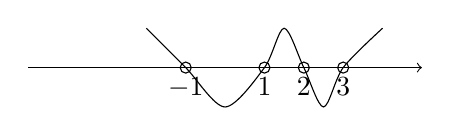
\begin{tikzpicture}[scale=0.5]
				    		\draw[black, ->] (-5, 0)--(5, 0);
				    		\draw[black] (-1, 0) circle (4pt) node[anchor=north] {$-1$};
				    		\draw[black] ( 1, 0) circle (4pt) node[anchor=north] {$1$};
				    		\draw[black] ( 2, 0) circle (4pt) node[anchor=north] {$2$};
				    		\draw[black] ( 3, 0) circle (4pt) node[anchor=north] {$3$};
				    		\draw[black] plot [smooth] coordinates {(4, 1) (3, 0) (2.5, -1) (2, 0) (1.5, 1) (1, 0) (0, -1) (-1, 0) (-2, 1)};
				    	\end{tikzpicture}
					$$

					因此解集为$(-1, 1)\cup(2, 3).$

					\textcolor{red}{\textbf{总结:图像不一定要完全精确,与$x$轴的关系正确即可.}}

				~\\

				\textbf{例二}:解不等式$\displaystyle (x-3)^3 (x-2)^2 (x-1) (x+1) \geq 0.$
					~\\

					与$x$轴交点为$x_1=-1, x_2=1, x_3=x_4=2, x_5=x_6=x_7=3.$

					$$
					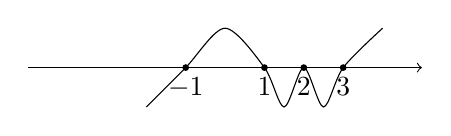
\begin{tikzpicture}[scale=0.5]
				    		\draw[black, ->] (-5, 0)--(5, 0);
				    		\filldraw[black] (-1, 0) circle (2pt) node[anchor=north] {$-1$};
				    		\filldraw[black] ( 1, 0) circle (2pt) node[anchor=north] {$1$};
				    		\filldraw[black] ( 2, 0) circle (2pt) node[anchor=north] {$2$};
				    		\filldraw[black] ( 3, 0) circle (2pt) node[anchor=north] {$3$};
				    		\draw[black] plot [smooth] coordinates {(4, 1) (3, 0) (2.5, -1) (2, 0) (1.5, -1) (1, 0) (0, 1) (-1, 0) (-2, -1)};
				    	\end{tikzpicture}
					$$

					因此解集为$[-1, 1]\cup\{2\}\cup[3, +\infty).$

					\textcolor{red}{\textbf{总结:(1) 奇穿偶不穿 (2) 注意数轴上$0$的点是否取.}}

				~\\

				\textbf{例三}:解不等式$\displaystyle (x-3)^3 (x-2)^2 (x-1) (x+1) \geq 0.$
					~\\

					与$x$轴交点为$x_1=-1, x_2=1, x_3=x_4=2, x_5=x_6=x_7=3.$

					$$
					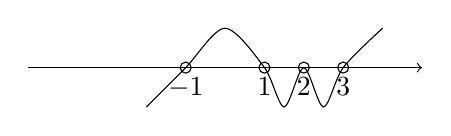
\begin{tikzpicture}[scale=0.5]
				    		\draw[black, ->] (-5, 0)--(5, 0);
				    		\draw[black] (-1, 0) circle (4pt) node[anchor=north] {$-1$};
				    		\draw[black] ( 1, 0) circle (4pt) node[anchor=north] {$1$};
				    		\draw[black] ( 2, 0) circle (4pt) node[anchor=north] {$2$};
				    		\draw[black] ( 3, 0) circle (4pt) node[anchor=north] {$3$};
				    		\draw[black] plot [smooth] coordinates {(4, 1) (3, 0) (2.5, -1) (2, 0) (1.5, -1) (1, 0) (0, 1) (-1, 0) (-2, -1)};
				    	\end{tikzpicture}
					$$

					因此解集为$(-\infty, -1) \cup (1, 2) \cup (2, 3).$

					\textcolor{red}{\textbf{总结:$\geq 0, \leq 0$类使用实心点,$>0, <0$使用实心点. 空心都不取,实心都取.}}

				~\\

				\textbf{例四}:解不等式$\displaystyle \frac{5x^2+12x-6}{3x^2+13x+4} \leq 1.$
					~\\

					化简,有$\displaystyle \frac{2x^2-x-10}{3x^2+13x+4} \leq 0$.

					于是有

					$$
					\left\{
					\begin{array}{rcl}
						(x+2)(2x-5)(x+4)(3x+1)&\leq&0\\
						(3x+1)(x+4)&\neq&0
					\end{array}
					\right.,
					$$

					与$x$轴交点为$x_1=-4, x_2=-2, x_3=-\frac{1}{3}, x_4=\frac{5}{2}.$

					$$
					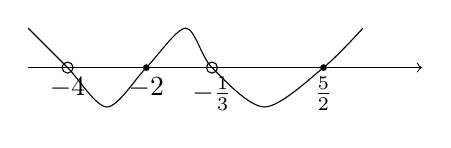
\begin{tikzpicture}[scale=0.5]
				    		\draw[black, ->] (-5, 0)--(5, 0);
				    		\draw[black] (-4, 0) circle (4pt) node[anchor=north] {$-4$};
				    		\filldraw[black] (-2, 0) circle (2pt) node[anchor=north] {$-2$};
				    		\draw[black] (-1/3, 0) circle (4pt) node[anchor=north] {$-\frac{1}{3}$};
				    		\filldraw[black] (5/2, 0) circle (2pt) node[anchor=north] {$\frac{5}{2}$};
				    		\draw[black] plot [smooth] coordinates {(7/2, 1) (5/2, 0) (1, -1) (-1/3, 0) (-1, 1) (-2, 0) (-3, -1) (-4, 0) (-5, 1)};
				    	\end{tikzpicture}
					$$

					解集为$(-4, -2]\cup\left(-\frac{1}{3}, \frac{5}{2}\right].$

					\textcolor{red}{\textbf{总结:分母不为$0$,使用空心点.}}

				~\\

				\textbf{例五}:$\displaystyle \frac{3x^2+2x+2}{x^2+x+1}>n$对一切$x\in\mathbf{R}$成立,$n\in\mathbf{N}^{*}$,求$n$.
					~\\

					$\because x^2+x+1 >0$

					$\therefore 3x^2+2x+2>n(x^2+x+1)$

					$\therefore (3-n)x^2+(2-n)x+2-n>0$

					$n=3$显然不成立,于是有:

					$$
					\left\{
					\begin{array}{rcl}
					3-n&>&0\\
					\Delta&<&0
					\end{array}
					\right.
					\Rightarrow
					n=1\text{ or }2.
					$$

					综上,$n\in\{1,2\}.$

					\textcolor{red}{\textbf{总结:当分母的正负性确定时,可直接利用乘法性质乘到不等式另一侧化为整式处理.}}

			\subsubsection{绝对值不等式的求解}
				\textbf{绝对值的运算}:
				$$
				|x|=\left\{
				\begin{array}{rcl}
				x&\text{for}&x>0\\
				0&\text{for}&x=0\\
				-x&\text{for}&x<0
				\end{array}
				\right..
				$$

				\textbf{绝对值的基本运算法则}:$\displaystyle|a+b|\neq|a|+|b|, |ab|=|a|\cdot|b|, \left|\frac{a}{b}\right|=\frac{|a|}{|b|}.$

				\textbf{$|f(x)|$$<$/$>$/$\leq$/$\geq$$a$类不等式的求解}:

				$$
				\begin{array}{ccccc}
					   &|f(x)|<a&|f(x)|>a&|f(x)|\leq a&|f(x)|\geq a\\
				    a>0&f(x)\in(-a, a)&f(x)\in(-\infty, -a)\cup(a, +\infty)&f(x)\in[-a, a]&f(x)\in(-\infty, -a]\cup[a, +\infty)\\
				    a=0&f(x)\in\emptyset&f(x)\in(-\infty, 0)\cup(0, +\infty)&f(x)\in\{0\}&f(x)\in\mathbf{R}\\
				    a<0&f(x)\in\emptyset&f(x)\in\mathbf{R}&f(x)\in\emptyset&f(x)\in\mathbf{R}\\
				\end{array}
				$$

				~\\

				\textbf{例一}:$\displaystyle \frac{1}{|2x-3|}\geq2.$
					~\\

					$$
					\left\{
					\begin{array}{rclcrccclcrcccl}
					2x-3&\neq&0&\Rightarrow&x&&\neq&&\frac{3}{2}\\
					|2x-3|&\leq&\frac{1}{2}&\Rightarrow&-\frac{1}{2}&\leq&2x-3&\leq&\frac{1}{2}&\Rightarrow&\frac{5}{4}&\leq&x&\leq&\frac{7}{4}
					\end{array}
					\right.
					\Rightarrow x\in\displaystyle\left[\frac{5}{4}, \frac{3}{2}\right)\cup\left(\frac{3}{2}, \frac{7}{4}\right].
					$$

					\textcolor{red}{\textbf{总结:(1) 切记分式的分母不等于0 (2) 绝对值恒大于等于零.}}

				~\\

				\textbf{$|f(x)|$$<$/$\leq$$|g(x)|$类不等式的求解}:

				$$|f(x)|<|g(x)| \Leftrightarrow f^2(x)<g^2(x) \Leftrightarrow [f(x)+g(x)]\cdot[f(x)-g(x)]<0,$$

				$$|f(x)|\leq|g(x)| \Leftrightarrow f^2(x)\leq g^2(x) \Leftrightarrow [f(x)+g(x)]\cdot[f(x)-g(x)]\leq 0.$$

				~\\

				\textbf{例二}:$|2x-1|>|x+2|.$
					~\\

					$\displaystyle (2x-1+x+2)(2x-1-x-2)>0\Rightarrow (3x+1)(x-3)>0 \Rightarrow x\in \left(-\infty, -\frac{1}{3}\right)\cup(3, +\infty).$

					\textcolor{red}{\textbf{总结:这题没啥好总结的,正常计算即可.}}

				~\\

				\textbf{例三}:$\displaystyle |x+2|>\frac{3x+14}{5}.$
					~\\

					\textbf{法一}:分两类讨论.

					\begin{enumerate}[label=$\arabic*^{\circ}$]
						\item $\left\{\begin{array}{rcl}x+2&>&0\\x+2&>&\displaystyle\frac{3x+4}{5}\end{array}\right.\Rightarrow x>2.$
						\item $\left\{\begin{array}{rcl}x+2&\leq&0\\-x-2&>&\displaystyle\frac{3x+4}{5}\end{array}\right.\Rightarrow x<-3.$
					\end{enumerate}

					于是有$x\in(-\infty, -3)\cup(2, +\infty).$

				~\\

				\textbf{$|f(x)|$$<$/$>$/$\leq$/$\geq$$g(x)$类不等式的求解}:

				$$|f(x)|<g(x)\Leftrightarrow -g(x)<f(x)<g(x), |f(x)|\leq g(x)\Leftrightarrow -g(x)\leq f(x)\leq g(x),$$

				$$|f(x)|>g(x)\Leftrightarrow g(x)<f(x) \text{ or } f(x)<-g(x), |f(x)|\geq g(x)\Leftrightarrow g(x)\leq f(x) \text{ or } f(x)\leq -g(x).$$
				~\\

				\textbf{例三}(续):$\displaystyle |x+2|>\frac{3x+14}{5}.$
				~\\

					\textbf{法二}:$\displaystyle x+2>\frac{3x+14}{5} \text{ or } x+2<-\frac{3x+14}{5} \Rightarrow x\in(-\infty, -3)\cup(2, +\infty).$

					\textcolor{red}{\textbf{总结:特法能更直接得到结论,通法对能用特法做的题同样适用.}}

				~\\

				\textbf{通法}:零点分段,去绝对值. \textbf{不等式、方程、函数均适用.}

				~\\

				\textbf{例四}:$|2x-1|-x<|x+3|+1.$
					~\\

					分三类讨论.

					\begin{enumerate}[label=$\arabic*^{\circ}$]
						\item $\left\{\begin{array}{rcl}x&<&-3\\1-2x-x&<&-3-x+1\end{array}\right.\Rightarrow x\in\emptyset.$
						\item $\left\{\begin{array}{rcccl}-3&\leq&x&<&\displaystyle\frac{1}{2}\\1-2x-x&&<&&x+3+1\end{array}\right.\Rightarrow x\in\displaystyle\left(-\frac{3}{4}, \frac{1}{2}\right).$
						\item $\left\{\begin{array}{rcl}x&\geq&\displaystyle\frac{1}{2}\\2x-1-x&<&x+3+1\end{array}\right.\Rightarrow x\in\displaystyle\left[\frac{1}{2}, +\infty\right).$
					\end{enumerate}

					综上,$x\in\displaystyle\left(-\frac{3}{4}, +\infty\right).$

					\textcolor{red}{\textbf{总结:通法的适用性更广,利用的是绝对值的定义.}}

			\subsubsection{补充:无理不等式的求解}
				\textbf{$\sqrt{f(x)}$$<$/$>$/$\leq$/$\geq$$a$类不等式的求解}:

				$$
				\begin{array}{ccccc}
					   &\sqrt{f(x)}<a&\sqrt{f(x)}>a&\sqrt{f(x)}\leq a&\sqrt{f(x)}\geq a\\
				    a>0&f(x)\in [0, a^2)&f(x)\in (a^2, +\infty)&f(x)\in [0, a^2]&f(x)\in [a^2, +\infty)\\
				    a=0&f(x)\in\emptyset&f(x)\in (0, +\infty)&f(x)\in\{0\}&f(x)\in[0, +\infty)\\
				    a<0&f(x)\in\emptyset&f(x)\in [0, +\infty)&f(x)\in\emptyset&f(x)\in [0, +\infty)\\
				\end{array}
				$$

				\textbf{$\sqrt{f(x)}$$<$/$>$/$\leq$/$\geq$$g(x)$类不等式的求解}:

				$$
				\sqrt{f(x)}<g(x)
				\Leftrightarrow
				\left\{
				\begin{array}{rcl}
				f(x)&\geq&0\\
				g(x)&>&0\\
				f(x)&<&g^2(x)\\
				\end{array}
				\right.,
				\sqrt{f(x)}\leq g(x)
				\Leftrightarrow
				\left\{
				\begin{array}{rcl}
				f(x)&\geq&0\\
				g(x)&\geq&0\\
				f(x)&\leq&g^2(x)\\
				\end{array}
				\right.,
				$$

				$$
				\sqrt{f(x)}>g(x)
				\Leftrightarrow
				\left\{
				\begin{array}{rcl}
				g(x)&\geq&0\\
				f(x)&>&g^2(x)\\
				\end{array}
				\right.
				\text{ or }
				\left\{
				\begin{array}{rcl}
				f(x)&\geq&0\\
				g(x)&<&0\\
				\end{array}
				\right.,
				$$

				$$
				\sqrt{f(x)}\geq g(x)
				\Leftrightarrow
				\left\{
				\begin{array}{rcl}
				g(x)&>&0\\
				f(x)&\geq&g^2(x)\\
				\end{array}
				\right.
				\text{ or }
				\left\{
				\begin{array}{rcl}
				f(x)&\geq&0\\
				g(x)&\leq&0\\
				\end{array}
				\right..
				$$

				\textbf{$\sqrt{f(x)}$$<$/$\leq$$\sqrt{g(x)}$类不等式的求解}:

				$$
				\sqrt{f(x)}<\sqrt{g(x)}
				\Leftrightarrow
				\left\{
				\begin{array}{rcl}
				f(x)&\geq&0\\
				f(x)&<&g(x)\\
				\end{array}
				\right.,
				\sqrt{f(x)}\leq\sqrt{g(x)}
				\Leftrightarrow
				\left\{
				\begin{array}{rcl}
				f(x)&\geq&0\\
				f(x)&\leq&g(x)\\
				\end{array}
				\right..
				$$

		\newpage
		\subsection{恒成立不等式及应用}
			\subsubsection{三角不等式}
				\textbf{三角不等式}:$|a|-|b|\leq|a+b|\leq|a|+|b|$,左边等号成立当且仅当$ab\leq 0$,右边等号成立当且仅当$ab\geq 0$,两边等号均成立当且仅当$ab=0$.

				证明三角不等式.

				$\because -|a|\leq a\leq |a|, -|b|\leq b\leq |b|$

				$\therefore -(|a|+|b|)\leq a+b\leq |a|+|b|$

				$\therefore |a+b|\leq|a|+|b|,$ 等号成立当且仅当$ab\geq 0.$

				$\because a=a+b-b$

				$\therefore |a|=|(a+b)+(-b)|\leq |a+b|+|b|$

				$\therefore |a|\leq|a+b|+|b|$

				$\therefore |a|-|b|\leq|a+b|,$ 等号成立当且仅当$ab\leq 0.$

				\textbf{三角不等式在多元上的推广}:$\displaystyle \left|\sum_{i=1}^{n} a_i\right|\leq \sum_{i=1}^{n}|a_i| (n \in \mathbf{N}, n\geq 2).$

				\textbf{三角不等式的推论}:$|a|-|b|\leq |a-b| \leq |a|+|b|.$

				\textbf{三角不等式的严格化推论}:$\left||a|-|b|\right|\leq|a+b|\leq|a|+|b|, \left||a|-|b|\right|\leq|a-b|\leq|a|-|b|.$

				\textbf{三角不等式的取等条件}:运算符号相同,$ab\geq 0$;运算符号相反,$ab\leq 0$;两边都要取到,$ab=0$.

				~\\

				\textbf{例一}:求$f(x)=|x-1|+|x-2|$的最小值.
					~\\

					$|x-1|+|x-2|=|x-1|+|2-x|\geq|(x-1)+(2-x)|=1,$

					当$(x-1)(2-x)\geq 0$即$1\leq 2\leq 2$时取等.

					$\therefore$当$x\in[1, 2]$时,$f_{\min}(x)=1.$

					\textcolor{red}{\textbf{总结:形如$f(x)=|x-a|+|x-b| (a>b)$的函数在$x\in[b, a]$时取到$f_{\min}(x)=a-b$.}}

				~\\

				\textbf{例二}:求$f(x)=|x-1|-|x+2|$的最大值.
					~\\

					$|x-1|-|x+2|\leq|(x-1)-(x+2)|=3,$

					当$(x-1)(x+2)\geq 0$且$|x-1|\geq |x+2|$时取等.

					$\therefore$当$x\in(-\infty, -2]$时,$f_{\max}(x)=3.$

					\textcolor{red}{\textbf{总结:形如$f(x)=|x-a|-|x-b| (a>b)$的函数在$x\in(-\infty, b]$时取到$f_{\max}(x)=a-b$.}}

			\subsubsection{基本不等式}
				\textbf{基本不等式1}:$\forall a, b \in \mathbf{R}: a^2+b^2\geq 2ab$,等号成立当且仅当$a=b$.

				\textbf{基本不等式2}:$\displaystyle \forall a, b \in \mathbf{R}^{+}: \frac{a+b}{2}\geq \sqrt{ab}$,等号成立当且仅当$a=b$.

				\textbf{基本不等式2的推广}:$\displaystyle \forall a, b \in \mathbf{R}^{+}: \frac{2}{\frac{1}{a}+\frac{1}{b}}\leq\sqrt{ab}\leq\frac{a+b}{2}\leq\sqrt{\frac{a^2+b^2}{2}}$,等号成立当且仅当$a=b$.(调和$\leq$几何$\leq$算术$\leq$平方)

				\textbf{基本不等式2的推广的推广}:$\displaystyle \forall a_1, a_2, \cdots, a_n \in \mathbf{R}^{+}: \frac{n}{\frac{1}{a_1}+\frac{1}{a_2}+\cdots+\frac{1}{a_n}}\leq\sqrt[n]{a_1 a_2 \cdots a_n}\leq\frac{a_1+a_2+\cdots+a_n}{n}\leq\sqrt{\frac{a_1^2+a_2^2+\cdots+a_n^2}{n}}$,等号成立当且仅当$a_1=a_2=\cdots=a_n.$

				\textbf{基本不等式2在负数上的推广}:$\displaystyle \forall a, b \in \mathbf{R}^{-}: \frac{a+b}{2}\leq -\sqrt{ab}$,等号成立当且仅当$a=b$.

				\textbf{基本不等式的应用}: (1) 一正:$a>0, b>0$ (2) 二定:积定和有最小值:$a+b\geq2\sqrt{ab}$;和定积有最大值:$ab\leq\left(\frac{a+b}{2}\right)^2$ (3) 三相等:考虑$=$能否取到.

				~\\

				\textbf{例一}:已知$x>0, a>0$.求$f(x)=x+\frac{a}{x}$的$f_{\min}(x)$并求出对应的$x$.
					~\\

					$\because x>0, a>0 \therefore \frac{a}{x}>0.$

					由基本不等式,有

					$$f(x)=x+\frac{a}{x}\geq2\sqrt{x\cdot\frac{a}{x}}=2\sqrt{a}.$$

					取等当且仅当$x=\frac{a}{x}$即$x=\pm\sqrt{a}$(舍负).

					于是有$f_{\min}(x)=f(\sqrt{a})=2\sqrt{a}.$

					\textcolor{red}{\textbf{总结:最基本的积定的直接应用.}}

				~\\

				\textbf{例二}:已知$a>0$.求$f(x)=x+\frac{a}{x}$的值域.
					~\\

					易得$x\neq0$.

					分两类讨论.

					\begin{enumerate}[label=$\arabic*^{\circ}$]
						\item
							$x>0,$

							由例一有$f_{\min}(x)=f(\sqrt{a})=2\sqrt{a}.$

						\item
							$x<0,$

							$\because x<0, a>0 \therefore \frac{a}{x}<0.$

							由基本不等式,有

							$$f(x)=x+\frac{a}{x}\leq-2\sqrt{x\cdot\frac{a}{x}}=-2\sqrt{a}.$$

							取等当且仅当$x=\frac{a}{x}$即$x=\pm\sqrt{a}$(舍正).

							于是有$f_{\max}(x)=f(-\sqrt{a})=-2\sqrt{a}.$

					\end{enumerate}

					综上,$f(x)$的值域为$\left(-\infty, -2\sqrt{a}\right]\cup\left[2\sqrt{a}, +\infty\right)$.

					\textcolor{red}{\textbf{总结:注意讨论$x$的正负号,利用基本不等式2及其在负数上的推广求值域.}}

				~\\

				\textbf{例三}:已知$x>1$.求$f(x)=x+\frac{1}{x-1}$的最小值.
					~\\

					$\because x>1 \therefore x>1>0, \frac{1}{x-1}>0.$

					由基本不等式,有

					$$f(x)-1=x+\frac{a}{x-1}-1=(x-1)+\frac{1}{x-1}\geq2\sqrt{(x-1)\cdot\frac{1}{x-1}}=2.$$

					取等当且仅当$x-1=\frac{1}{x-1}$即$x-1=\pm1$即$x=\pm1+1=2$或$0$(舍).

					于是有$f_{\min}(x)=f(2)=3.$

					\textcolor{red}{\textbf{总结:构造积定,变为基本不等式的形式.}}

				~\\

				\textbf{例四}:求$\displaystyle f(x)=\frac{x^2+x+1}{x+1}$的值域.
					~\\

					$f(x)=x+\frac{1}{x+1}.$

					易得$x\neq-1$.

					分两类讨论.

					\begin{enumerate}[label=$\arabic*^{\circ}$]
						\item
							$x>-1,$

							$\because x>-1 \therefore x+1>0, \frac{1}{x+1}>0.$

							由基本不等式,有

							$$f(x)+1=x+\frac{1}{x+1}+1=(x+1)+\frac{1}{x+1}\geq2\sqrt{(x+1)\cdot\frac{1}{x+1}}=2.$$

							取等当且仅当$x+1=\frac{1}{x+1}$即$x+1=\pm1$即$x=0$或$-2$(舍).

							于是有$f_{\min}(x)=f(0)=1.$

						\item
							$x<-1,$

							$\because x<-1 \therefore x+1<0, \frac{1}{x+1}<0.$

							由基本不等式,有

							$$f(x)+1=x+\frac{1}{x+1}+1=(x+1)+\frac{1}{x+1}\leq-2\sqrt{(x+1)\cdot\frac{1}{x+1}}=-2.$$

							取等当且仅当$x+1=\frac{1}{x+1}$即$x+1=\pm1$即$x=-2$或$0$(舍).

							于是有$f_{\max}(x)=f(-2)=-3.$

					\end{enumerate}

					综上,$f(x)$的值域为$\left(-\infty, -3\right]\cup\left[1,+\infty\right)$.

					\textcolor{red}{\textbf{总结:分子次数比分母高(常见为二次和一次),分子可选择换元进行求解.}}

				~\\

				\textbf{例五}:求$\displaystyle f(x)=\frac{2x}{x^2+x+1}$的值域.
					~\\

					分两类讨论.

					\begin{enumerate}[label=$\arabic*^{\circ}$]
						\item
							$x=0,$

							$f(0)=0$

						\item
							$x\neq 0,$

							$\displaystyle f(x)=\frac{2}{x+1+\frac{1}{x}}.$

							由(2)有$g(x)=x+\frac{1}{x}$的值域为$\left(-\infty,-2\right]\cup\left[2,+\infty\right).$

							$\therefore g(x)+1$的值域为$\left(-\infty,-1\right]\cup\left[3,+\infty\right).$

							$\therefore \frac{1}{g(x)+1}$的值域为$\left[-1,0\right)\cup\left(0,\frac{1}{3}\right].$

							$\therefore \frac{2}{g(x)+1}=f(x)$的值域为$\left[-2,0\right)\cup\left(0,\frac{2}{3}\right].$

					\end{enumerate}

					综上,$f(x)$的值域为$\left[-2,\frac{2}{3}\right].$

					\textcolor{red}{\textbf{总结:分母次数比分子高(常见为一次和二次),勿忘讨论分子为0,分子除到分母上.}}

				~\\

				\textbf{例六}:求$\displaystyle f(x)=\frac{x^2+3x+1}{x^2+x+1}$的值域.
					~\\

					$\displaystyle \frac{x^2+3x+1}{x^2+x+1}=1+\frac{2x}{x^2+x+1}.$

					由例五有$f(x)$的值域为$\left[-1,\frac{5}{3}\right].$

					\textcolor{red}{\textbf{总结:分母次数与分子相同(常见为二次和二次),分子滚分母,分离整系数.}}

				~\\

				\textbf{例七}:求$\displaystyle f(x)=\frac{x^4+x^2+1}{x^2+1}$的值域.
					~\\

					令$t=x^2 (t\geq 0)$,则有$\displaystyle \frac{x^4+x^2+1}{x^2+1}=\frac{t^2+t+1}{t+1}.$

					由例四有$f(x)$的值域为$\left[1, +\infty\right).$

					\textcolor{red}{\textbf{总结:分母分子高次,换元降次.}}

				~\\

				\textbf{例八}:已知$0<x<1$,求函数$f(x)=x(1-x)$的最大值.
					~\\

					$\because 0<x<1$

					$\therefore 0<1-x<1$

					$\therefore \displaystyle f(x)=x(1-x)\leq \left(\frac{x+1-x}{2}\right)^2=\frac{1}{4}$,等号成立当且仅当$x=1-x$即$x=\displaystyle \frac{1}{2}$.

					$\therefore \displaystyle f_{\max}(x)=f\left(\frac{1}{2}\right)=\frac{1}{4}.$

					\textcolor{red}{\textbf{总结:最基本的和定的直接应用.}}

				~\\

				\textbf{例九}:已知$\displaystyle 0<x<\frac{1}{2}$,求函数$f(x)=x(1-2x)$的最大值.
					~\\

					$\because \displaystyle 0<x<\frac{1}{2}$

					$\therefore 0<1-2x<1$

					$\therefore \displaystyle f(x)=x(1-2x)=\frac{1}{2}\cdots 2x(1-2x) \leq \frac{1}{2} \left(\frac{2x+1-2x}{2}\right)^2=\frac{1}{8}$,等号成立当且仅当$2x=1-2x$即$x=\frac{1}{4}$.

					$\therefore \displaystyle f_{\max}(x)=f\left(\frac{1}{4}\right)=\frac{1}{8}.$

					\textcolor{red}{\textbf{总结:构造和定,变为基本不等式的形式.}}

				~\\

				\textbf{例十}:已知$a, b, x, y \in \mathbf{R}^{+}, \displaystyle \frac{a}{x}+\frac{b}{y}=1.$
					\begin{enumerate}[label=(\arabic*)]
						\item $a=2, b=1$, 求$(x+y)_{\min}$.
						\item 若$a+b=5$且$(x+y)_{\min}=9$, 求$a, b$.
					\end{enumerate}

					\begin{enumerate}[label=(\arabic*)]
						\item $a=2, b=1$, 求$(x+y)_{\min}$.

							\textcolor{red}{\textbf{典型错误:$\displaystyle1=\frac{2}{x}+\frac{1}{y}\geq2\sqrt{\frac{2}{x}\cdot\frac{1}{y}}\Rightarrow xy\geq 8 \Rightarrow x+y\geq 2\sqrt{xy}\geq 4\sqrt{2}.$}}

							\textcolor{red}{\textbf{两次使用基本不等式一定要注意等号成立条件是否能同时取到!}}

							$\because x, y\in\mathbf{R}^{+}$

							$\therefore \displaystyle x+y=(x+y)\left(\frac{2}{x}+\frac{1}{y}\right)=3+\frac{x}{y}+\frac{2y}{x}\geq3+\sqrt{\frac{x}{y}\cdot\frac{2y}{x}}=3+2\sqrt{2},$

							等号成立当且仅当$\displaystyle \frac{2y}{x}=\frac{x}{y} \text{ and } \frac{2}{x}+\frac{1}{y}=1$即$x=2+\sqrt{2}, y=1+\sqrt{2}.$

							$\therefore x=2+\sqrt{2}, y=\sqrt{2}+1$时,$(x+y)_{\min}=3+2\sqrt{2}.$

						\item 若$a+b=5$且$(x+y)_{\min}=9$, 求$a, b$.

							$\displaystyle (x+y)\left(\frac{a}{x}+\frac{b}{y}\right)=a+b+\frac{ay}{x}+\frac{bx}{y}\geq a+b+2\sqrt{ab}=5+2\sqrt{ab}=9$,

							等号成立当且仅当$bx^2=ay^2$时取等.

							$$
							\left\{
							\begin{array}{rcl}
								\sqrt{ab}&=&2\\
								a+b&=&5\\
							\end{array}
							\right.
							\Rightarrow
							\left\{
							\begin{array}{rcl}
								a&=&1\\
								b&=&4\\
							\end{array}
							\right.
							\text{ or }
							\left\{
							\begin{array}{rcl}
								a&=&4\\
								b&=&1\\
							\end{array}
							\right..
							$$

							验证等号成立条件,对应即为$y=2x$或$x=2y$时等号成立.

							$\therefore (a,b)=(1,4) \text{ or } (4,1).$

					\end{enumerate}

					\textcolor{red}{\textbf{总结:在无法直接转换为基本不等式时,可考虑使用“1”进行代换.}}

				~\\

				\textbf{例十一}:$\displaystyle (x+y)\left(\frac{1}{x}+\frac{a}{y}\right)\geq 9$对任意正实数$x, y$恒成立,求正实数$a$的最小值.
					~\\

					即$\text{左边}_{\min} \geq 9$.

					$\displaystyle a+1+\frac{y}{x}+\frac{xa}{y}\geq a+1+2\sqrt{a}\geq 9$,等号成立当且仅当$ax^2=y^2.$

					有$(\sqrt{a}+1)^2\geq 9 \Rightarrow \sqrt{a}\geq 2 \Rightarrow a\geq 4.$

					当$a=4$时,验证等号成立条件即为$x=2y$.

					于是$a_{\min}=4.$

					\textcolor{red}{\textbf{总结:恒大于等于/小于等于问题考虑最小值/最大值恒大于等于/小于等于,可以考虑使用基本不等式求解.}}

				~\\

				\textbf{例十二}:$(k^2+k+1)x^2-2(a+k)^2x+k^2+3ak+b=0$对任意实数$k$恒有根$1$. 求:
					\begin{enumerate}[label=(\arabic*)]
						\item $a, b$
						\item $k$变化时,另一根的变化范围.
					\end{enumerate}

					\begin{enumerate}[label=(\arabic*)]
						\item $a, b$

							代入$x=1$有: $(1-a)k+1-2a^2+b=0$对$k\in\mathbf{R}$恒成立,有:

							$$
							\left\{
							\begin{array}{rcl}
								1-a&=&0\\
								1-2a^2+b&=&0
							\end{array}
							\right.
							\Rightarrow
							\left\{
							\begin{array}{rcl}
								a&=&1\\
								b&=&1\\
							\end{array}
							\right..
							$$

						\item $k$变化时,另一根的变化范围.

							设另一根为$x_2$,由Vieta定理,有:

							$\displaystyle x_2\cdot1=\frac{k^2+3k+1}{k^2+k+1}=1+\frac{2k}{k^2+k+1}.$

							由例五有$\displaystyle x_2\in\left[-1, \frac{5}{3}\right].$

					\end{enumerate}

					\textcolor{red}{\textbf{总结:(1) 对什么变量恒成立,什么就是主元 (2) “$0=0$”类问题,主元的每个系数均对应相同 (3) Vieta定理可用来确定根的范围.}}

				~\\

				\textbf{例十三}:$(kx-k^2-4)(x-4)>0, k\in\mathbf{R}.$
					\begin{enumerate}[label=(\arabic*)]
						\item $k$变化时,求解集$A$.
						\item 若$A\cap\mathbf{Z}=B,$探究$B$能否为有限集?若能,求$B$中元素最少的$k$的取值并用列举法表示$B$.
					\end{enumerate}

					\begin{enumerate}[label=(\arabic*)]
						\item $k$变化时,求解集$A$.

							$\displaystyle \frac{k^2+4}{k}=k+\frac{4}{k}\in(-\infty, 4]\cup[4, +\infty).$

							\begin{enumerate}[label=$\arabic*^{\circ}$]
								\item $k=0, A=(-\infty, 4)$.
								\item $k>0, \displaystyle\frac{k^2+4}{k}\geq 4, A=(-\infty, 4)\cup\left(\frac{k^2+4}{k}, +\infty\right).$
								\item $k<0, \displaystyle\frac{k^2+4}{k}\leq -4 < 4, A=\left(\frac{k^2+4}{k}, 4\right).$
							\end{enumerate}

							综上,当$\displaystyle k\in(-\infty, 0), A=\left(\frac{k^2+4}{k}, 4\right)$;当$\displaystyle k=0, A=(-\infty, 4)$;当$\displaystyle k\in(0, +\infty), A=(-\infty, 4)\cup\left(\frac{k^2+4}{k}, +\infty\right).$

						\item 若$A\cap\mathbf{Z}=B,$探究$B$能否为有限集?若能,求$B$中元素最少的$k$的取值并用列举法表示$B$.

							由(1)有$k\geq 0, B$为无限集;当$k<0, B$为有限集.

							$\displaystyle \therefore k<0, A=\left(\frac{k^2+4}{k}, 4\right).$

							$\displaystyle k+\frac{4}{k}\leq-2\sqrt{k\cdot\frac{4}{k}}=-4$,等号成立当且仅当$k=-2$.

							当$k=-2$,$A=(-4, 4)$最短.

							此时$B$中元素最少,$B=\{-3, -2, -1, 0, 1, 2, 3\}.$

					\end{enumerate}

					\textcolor{red}{\textbf{总结:(1) 基本不等式可帮助确定二次方程两根大小关系和最值相关问题 (2) “探究”问题无论结果如何均需写出过程.}}

		\newpage
		\subsection{不等式的证明}
			\subsubsection{比较法}
				\textbf{比较法一般步骤}:(1) 作差(商) (2) 变形 (3) 判断.

				~\\

				\textbf{例一}:求证$a^2+b^2\geq ab+a+b-1$.
					~\\

					\textbf{法一}:作差.

					$$
					\begin{array}{cl}
						&(a^2+b^2)-(ab+a+b-1)\\
					=	&\displaystyle \frac{1}{2}\left[(a-b)^2+(a-1)^2+(b-1)^2\right]\\
					\geq&0.
					\end{array}
					$$

					即$a^2+b^2\geq ab+a+b-1$.

					\textbf{法二}:构造二次函数.

					记$f(a)=a^2-(b+1)a+b^2-b+1.$

					$\Delta=(b+1)^2-4(b^2-b+1)=-3(b-1)^3\leq 0.$

					又二次项系数为$1$恒为正,有$f(a)\geq 0$,即$a^2+b^2\geq ab+a+b-1$.

					\textcolor{red}{\textbf{总结:(1) 作差法是万!能!的! (2) 构造二次函数,利用二次函数的最小值同样也是常见的求最值/证明不等式恒成立的方法.}}

				~\\

				\textbf{例二}:已知$a, b, m\in\mathbf{R}^{+}, a<b,$求证:$\displaystyle\frac{a+m}{b+m}>\frac{a}{b}.$
					~\\

					$\displaystyle \frac{a+m}{b+m}-\frac{a}{b}=\frac{(b-a)m}{b(b+m)}.$

					$\because b>0, b+m>0, b-a>0, m>0$

					$\therefore \displaystyle \frac{(b-a)m}{b(b+m)}>0$

					$\therefore \displaystyle \frac{a+m}{b+m}>\frac{a}{b}.$

					\textcolor{red}{\textbf{总结:作差法一般变形为平方、绝对值、根式(恒成立)或多个代数式的乘积,根据每项的正负性证明差的正负性.}}

			\subsubsection{综合法}
				\textbf{综合法}:由条件分析.

				\textbf{例}:已知$a, b, c$为不全相等的正数. 求证:$\displaystyle \frac{b+c-a}{a}+\frac{c-a-b}{b}+\frac{a+b-c}{c}>3$.
					~\\

					左边$=\displaystyle\left(\frac{b}{a}+\frac{a}{b}\right)+\left(\frac{c}{b}+\frac{b}{c}\right)+\left(\frac{a}{c}+\frac{c}{a}\right)-3.$

					$\because a, b, c$为不全相等的正数

					$\therefore \frac{b}{a}+\frac{a}{b}\geq 2, \frac{c}{b}+\frac{b}{c}\geq 2, \frac{a}{c}+\frac{c}{a}\geq 2$,等号不能同时取到.

					$\therefore$左边$>3$.

					\textcolor{red}{\textbf{总结:(1) 综合法一般用在一步步化简方法比较明显的题目上 (2) 基本不等式的等号不同时取到是去除等号的很重要的一种方法.}}

			\subsubsection{分析法}
				\textbf{分析法}:从结论推到已知. \textbf{注意格式.}

				\textbf{例}:已知$a>b>0$,求证:$\displaystyle \frac{(a-b)^2}{8a}<\frac{a+b}{2}-\sqrt{ab}<\frac{(a-b)^2}{8b}.$
					~\\

					欲证$\displaystyle \frac{(a-b)^2}{8a}<\frac{a+b}{2}-\sqrt{ab}<\frac{(a-b)^2}{8b}$

					只需证$\displaystyle \frac{(a-b)^2}{4a}<a+b-2\sqrt{ab}<\frac{(a-b)^2}{4b}$

					只需证$\displaystyle \left(\frac{a-b}{2\sqrt{a}}\right)^2<\left(\sqrt{a}-\sqrt{b}\right)^2<\left(\frac{a-b}{2\sqrt{b}}\right)^2$

					只需证$\displaystyle \frac{a-b}{2\sqrt{a}}<\sqrt{a}-\sqrt{b}<\frac{a-b}{2\sqrt{b}}$

					即证$\displaystyle \frac{\sqrt{a}+\sqrt{b}}{2\sqrt{a}}<1<\frac{\sqrt{a}+\sqrt{b}}{2\sqrt{b}}$

					即证$\displaystyle 1+\frac{\sqrt{b}}{\sqrt{a}}<2<1+\frac{\sqrt{a}}{\sqrt{b}}$

					即证$\displaystyle \frac{\sqrt{b}}{\sqrt{a}}<1<\frac{\sqrt{a}}{\sqrt{b}}$

					$\because a>b>0$

					$\therefore \sqrt{a}>\sqrt{b}>0$

					$\displaystyle \therefore\frac{\sqrt{b}}{\sqrt{a}}<1<\frac{\sqrt{a}}{\sqrt{b}}$成立

					故原不等式成立.

					\textcolor{red}{\textbf{总结:分析法一般用在一步步化简方法不明显,从结论分析会比较容易的难题上,现阶段很少出现,主要为后面的函数综合题作准备.}}

			\subsubsection{反证法}
				\textbf{例}:$f(x)=x^2+px+q$. 证明$|f(1)|, |f(2)|, |f(3)|$至少一个不小于$\displaystyle\frac{1}{2}$.
					~\\

					假设三者均小于$\displaystyle\frac{1}{2}$

					$|f(1)|=|p+q+1|, |f(2)|=|2p+q+4|, |f(3)|=|3p+q+9|.$

					\textbf{法一}:$\because f(1)=p+q+1, f(2)=2p+q+4$

					$\therefore p=f(2)-f(1)-3, q=2f(1)-f(2)+2$

					$\displaystyle \therefore |f(3)|=|2f(2)-f(1)+2|\geq 2f(2)-f(1)+2>-2\times \frac{1}{2}-\frac{1}{2}+2=\frac{1}{2}$与假设矛盾.

					于是$|f(1)|, |f(2)|, |f(3)|$至少一个不小于$\displaystyle\frac{1}{2}$.

					\textbf{法二}:$f(1)+f(3)-2f(2)=2$.

					但$|f(1)+f(3)-2f(2)|\leq|f(1)|+|f(3)|+2|f(2)|<\frac{1}{2}+\frac{1}{2}+2\times\frac{1}{2}=2$与之矛盾.

					于是$|f(1)|, |f(2)|, |f(3)|$至少一个不小于$\displaystyle\frac{1}{2}$.

					\textcolor{red}{\textbf{总结:反证法一般用在求证内容带有“存在”等词的题,一般正面证明较为困难,使用反证法即为“都不”,推出矛盾较为容易.}}

			\subsubsection{放缩法}
				\textbf{例}:求证:$\displaystyle \frac{|a+b|}{1+|a+b|}\leq\frac{|a|}{1+|a|}+\frac{|b|}{1+|b|}.$

					\begin{enumerate}[label=$\arabic*^{\circ}$]
						\item $|a+b|=0$显然成立.
						\item $|a+b| \neq 0$, $0<|a+b|\leq|a|+|b| \Rightarrow \displaystyle \frac{1}{|a+b|}\geq\frac{1}{|a|+|b|}.$

							$$
							\begin{array}{rcl}
								\text{左边}&=&\displaystyle \frac{|a+b|}{1+|a+b|}\\
								&=&\displaystyle \frac{1}{\frac{1}{|a+b|}+1}\\
								&\leq&\displaystyle \frac{1}{\frac{1}{|a|+|b|}+1}\\
								&=&\displaystyle \frac{|a|+|b|}{1+|a|+|b|}\\
								&=&\displaystyle \frac{|a|}{1+|a|+|b|} + \frac{|b|}{1+|a|+|b|}\\
								&\leq&\displaystyle \frac{|a|}{1+|a|}+\frac{|b|}{1+|b|}.
							\end{array}
							$$
					\end{enumerate}

					于是得证.

					\textcolor{red}{\textbf{总结:放缩法常见于其它证明方法当中,且需要适当的技巧和熟练度.}}

\end{document}